\documentclass[a4paper]{jreport}
%##########################################################################################
\input{00_version}
\title{{\Huge USERS GUIDE for SCALE-GM\\
        \vspace{2cm}{\Large Version \version} }}
\vspace{3cm}
\author{\Large Team SCALE\\ UGC working group}
\vspace{3cm}
\date{\西暦{\today}}
\vspace{3cm}

\usepackage[dvipdfmx]{graphicx, color}
\usepackage[dvipdfmx]{hyperref}
\usepackage{float}
%\usepackage{amsmath}
%\usepackage{ascmac}
%\usepackage[round]{natbib}
\usepackage{tabularx}
\usepackage{color}
\usepackage{colortbl}
%\usepackage{fancybox}
\usepackage{url}
\usepackage{pxjahyper}
\hypersetup{% options for hyperref
 bookmarksopen=true,
 bookmarksnumbered=true,
 colorlinks=true,
% linkcolor=red,
 linkcolor=cyan,
 citecolor=cyan,
 urlcolor=cyan,
}
\usepackage[top=30mm,bottom=35mm,left=30mm,right=30mm]{geometry}
\renewcommand{\thefootnote}{*\arabic{footnote})}

\begin{document}
\maketitle

\clearpage
\tableofcontents

\chapter{概要}\label{chap:overview}
%###############################################################################
\section{はじめに}
%-------------------------------------------------------------------------------

本書は``SCALE USERS GUIDE''の別冊として
SCALEライブラリパッケージに含まれる全球モデル SCALE-Global Model(GM) の利用方法を説明する。
SCALE-GMはSCALEライブラリを用いて構築された全球大気モデルのことを指す。
SCALE-GMの実行手順についてDCMIP2016実験を用いて解説する。
SCALEライブラリの概要については``SCALE USERS GUIDE''の第1章を参照されたい。


SCALE-GMは、Nonhydrostatic ICosahedral Atmospheric Model (NICAM)として開発された
正二十面体格子の力学コアをライブラリとして再構成したものでる。
現行のSCALE-GMは力学コアの理想実験を実行することができる。
%物理パッケージを含めたNICAMは、海洋開発研究機構(JAMSTEC)、東京大学大気海洋研究所(AORI)と
%理化学研究所計算科学研究機構(AICS)が共同開発している。


%\textcolor{red}{[英語版未対応-------ここから]}

ここで、SCALE-GMの力学コアについて簡潔に説明する。
予報変数は、密度、運動量、全エネルギー(運動エネルギー+内部エネルギー)、及び凝結物等のトレーサーである。
音波は水平方向には陽解法で計算され、鉛直方向には陰解法で計算される(HEVI)。
格子のトポロジーは正二十面体をベースにしており、水平方向にはArakawa A-gridの格子点配置が適用されている。
したがって、全ての予報変数は六角形セルの中心に位置している。
水平方向のオペレーターの離散化には有限体積法を用いている。
鉛直方向にはLorenzタイプのスタッガード格子が利用されている。
正二十面体格子の最適化にはバネ格子法(Tomita et al. 2002)を用いて最適化されており、特定の場所に
格子点を集めて局所的に高解像度化させるストレッチ格子(Tomita et al. 2008)も利用できる。
有限体積法による水平離散化においては、2次精度のdivergenceとgradientが使用されている(Tomita et al. 2001)。
トレーサー移流においては、線形再構築を用いた上流型の移流スキーム(Miura 2007)が用いられている。
時間積分に関しては、3段、もしくは2段のルンゲ・クッタスキームを用いることができる。
また、計算安定性のための数値粘性として、4次の高次粘性スキームが実装されている。

SCALE-GMの力学コアのさらなる詳細については、Tomita and Satoh (2004)やSatoh et al. (2008)
%NICAM.jp (\url{http://nicam.jp/})
を参照されたい。

%\textcolor{red}{[英語版未対応-------ここまで]}

\section{SCALE-GMにおける用語について}
%-------------------------------------------------------------------------------

 \begin{itemize}
   \item g-level (grid level): 正二十面体は正三角形で面が構成されているが、元の正二十面体から
正三角形が何度分割されたか、その分割回数を示す整数である。したがって、g-levelが大きいと格子点数が増え、
水平格子間隔が小さくなることに相当する。g-level 1 は元の正二十面体を意味する。
g-level 4以上の格子を使用することを推奨する。
おおよその水平格子間隔は、g-level 4=480 km、5=240 km、6=120 km、7=60 km、8=30 kmである。
   \item r-level (region level): 正二十面体において正三角形を2つ組み合わせた菱型のタイルをregionと
呼び、元の正二十面体から菱型が何度分割されたか、その分割回数を示す整数である。
r-levelが0の場合、10個の菱型(region)が存在する。1つのregionに含まれる格子点上の計算を1つのMPIプロセスが
担当する。したがって、r-level=0の場合、最大並列数は10プロセスである。r-level 1であれば40プロセス、
r-level 2であれば、160プロセスと並列できるプロセス数が増加する。ただ、r-levelを上げることは、Haloに含まれる
格子点数を増やすことになるので、低いg-level(低解像度)において、高いr-levelを使用することは避けること。
 \end{itemize}

\begin{figure}[H]
\centering
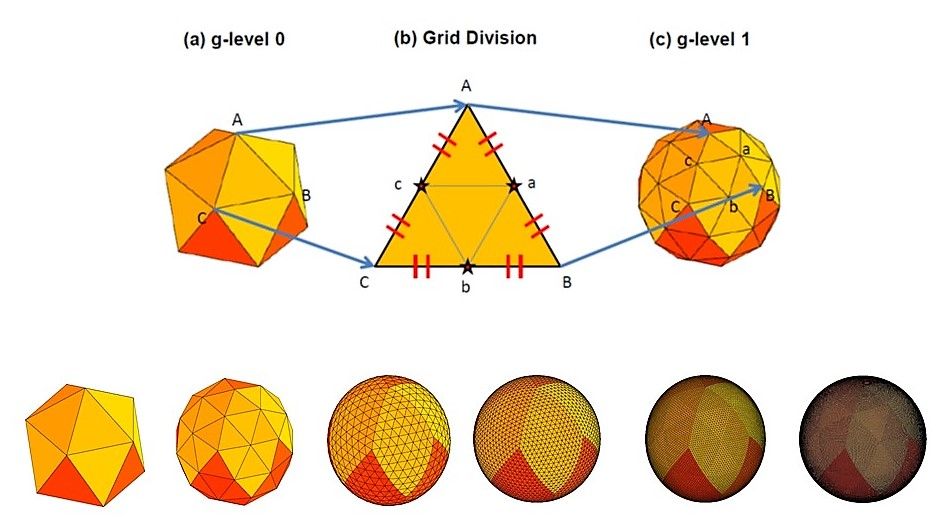
\includegraphics[width=15cm]{../../figure/g-level_concept.jpg}
\caption{g-levelの概念図}
\centering
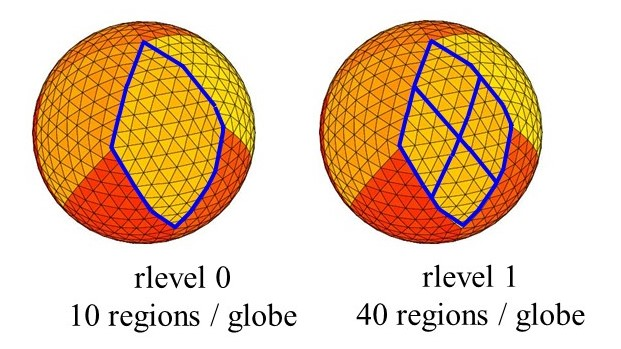
\includegraphics[width=10cm]{../../figure/r-level_concept.jpg}
\caption{r-levelの概念図}
\end{figure}

\textcolor{red}{[要検討: ここに、g-levelとr-levelを説明するための適切な図を追
    加する必要がある:とりあず佐藤さんの発表資料より拝借!さらにHALOを説明する図
    もある方が良い]}


\section{表記上の注意}
%-------------------------------------------------------------------------------
 \begin{itemize}
   \item 本書の説明はbash環境を想定している。
         tcsh環境においては、文中のコマンドの``export''を``setenv''に読み替える必要がある。
         (例. \verb|> setenv SCALE_SYS "Linux64-gnu-ompi"|)
   \item ``\verb|>|'' の記号は端末においてコマンドを実行することを意味する。
   \item 文中のゴシック体は標準出力の結果であることを意味する。
%   \item \$\{TOP\} は   \verb|scale/scale-gm| のディレクトリを指す。
%   \item \$\{ROOT\} は  \verb|scale| のディレクトリを指す。
 \end{itemize}



\chapter{クイックスタート}\label{chap:quickstart}
\section{Quick Start}
%###############################################################################

\subsection{Preparation}
%-------------------------------------------------------------------------------
Please see the Chapter 2.1 and 2.2 of ``SCALE USERS GUIDE''
as to the details of required system environment, library, and settings of environmental parameters.
Required libraries for SCALE-GM is same as SCALE-RM; HDF5, NetCDF, and MPI.

\subsection{Compile}
%-------------------------------------------------------------------------------
Please refer the Chapter 2.3.1 of ``SCALE USERS GUIDE'' for how to get the source code
and the Chapter 2.3.2 for the system environmental parameters.
Change directly to test case directly, for example,

\begin{verbatim}
  > cd ${TOP}/src
\end{verbatim}

\noindent Compile the program using make command.
\begin{verbatim}
  > make -j 4
\end{verbatim}
When the compile is finished correctly,
a "\verb|scale-gm|" is created in the directly of \verb|${ROOT}/bin|,
which is an executable binary of SCALE-GM.

\begin{itemize}
  \item[*] The number of -j option is a number of parallel compile processes.
   To reduce elapsed time of compile, you can specify the number
   as more than two. We recommend 2 $\sim$ 8 for the -j option.
\end{itemize}

\subsection{Run experiments}
%-------------------------------------------------------------------------------
\subsubsection{Test cases}

\noindent Inside the \${TOP}/test/case directory, you will find various test cases.
For example, the cases based on DCMIP2016 are shown in Table 1.

 \begin{table}[b]
 \begin{center}
 \caption{Corresponding test cases}
 \begin{tabularx}{150mm}{|l|X|} \hline
 \rowcolor[gray]{0.9} test case name in NICAM & test case type \\ \hline
  DCMIP2016-11 & moist baroclinic wave test (161)       \\ \hline
  DCMIP2016-12 & idealized tropical cyclone test (162)  \\ \hline
  DCMIP2016-13 & supercell test (163)                   \\ \hline
 \end{tabularx}
 \end{center}
 \end{table}


\subsubsection{How to run}

The script for job execution depends on the system.
SCALE-GM has a function, which produces scripts in consideration
of the difference of system environment.
Move to a directory of test case and then type
to create a job script and a script for post-processing;

 \begin{verbatim}
   > make jobshell
 \end{verbatim}

To run the model, type following command;

 \begin{verbatim}
   > make run
 \end{verbatim}

The test experiment will be started.

\subsection{Post process}
%-------------------------------------------------------------------------------
 After finish of test run, create the lat-lon grid data from
 the original icosahedral grid data.
 Before submit a job of post process, edit \verb|ico2ll_netcdf.sh|
 following your experimental settings.
 \begin{verbatim}
   > vi ico2ll_netcdf.sh

   [at Line 22]
   # User Settings
   # ---------------------------------------------------------------------

   glev=5          # g-level of original grid
   case=161        # test case number
   out_intev='day' # output interval (format: "1hr", "6hr", "day", "100s")
 \end{verbatim}

 \noindent If the job script is OK, submit a job to the machine.
 \begin{verbatim}
   sh ico2ll_netcdf.sh
 \end{verbatim}

% \begin{verbatim}
%   > bsub < ico2ll_netcdf.sh
% \end{verbatim}

 \noindent The netcdf format data such as "\verb|nicam.161.200.L30.interp_latlon.nc|"
 is created by an "ico2ll" post-process program.



\chapter{実験設定とモデル設定の変更方法}\label{chap:settings}
\section{Change Model Configurations}
%###############################################################################
 {\sf Terms}
 \begin{itemize}
   \item g-level (grid level): number of subdivision times of the grid from the original icosahedron.
         the number starts from 1, we recommend to use the number larger than 4.
   \item r-level (region level): number of subdivision times of the region(tile)
         from the original icosahedron. When r-level = 0, we have ten regions(tiles).
         At that time, the number of available maximum MPI processes is ten.
 \end{itemize}

\subsection{Change the Test Case}
%-------------------------------------------------------------------------------

 \noindent In this section, detail of the configurations of three experiments
 in DCMIP2016 are described. Each configuration set in the directory of \verb|${TOP}/test/case|
 is ready to go. At the first step, please use these sets as it is.

\subsubsection{preparing directory}
 Change to the directory of target case. If you want to run test case 162,
 change to \verb|${TOP}/test/case/DCMIP2016-12/|. After that, make a directory.
 The directory of gl05rl00z30pe40 already may exists, we assume create it newly.
 \begin{verbatim}
    > mkdir gl05rl00z30pe40
    > cd    gl05rl00z30pe40
 \end{verbatim}

 \noindent Copy Makefile and configuration file from another directory
 of DCMIP2016 to the new direcotory, for example DCMIP2016-11.
 \begin{verbatim}
    > cp ../../DCMIP2016-11/gl05rl00z30pe10/Makefile       ./
    > cp ../../DCMIP2016-11/gl05rl00z30pe10/nhm_driver.cnf ./
 \end{verbatim}

\subsubsection{Edit configuration file: nhm\_driver.cnf}

 %--------------------
 \vspace{0.5cm}
 \noindent {\large{\sf edit for test case 161: moist baroclinic wave}}

 (symbols "\verb|<--|" means changed parameters)
 \begin{verbatim}
    > vi nhm_driver.cnf
     * snip *

     &RUNCONFPARAM
       RUNNAME        = 'DCMIP2016-11',      <--
       NDIFF_LOCATION = 'IN_LARGE_STEP2',
       THUBURN_LIM    = .true.,
       RAIN_TYPE      = "WARM",
       AF_TYPE        = 'DCMIP',
     /

     * snip *

     &DYCORETESTPARAM
       init_type   = 'Jablonowski-Moist',    <--
       test_case   = '1',                    <--
       chemtracer  = .true.,                 <--
       prs_rebuild = .false.,
     /

     * snip *

     &FORCING_DCMIP_PARAM
       SET_DCMIP2016_11 = .true.,            <--
     /

     * snip *
 \end{verbatim}

 \noindent \textcolor{blue}{{\sf Note}}
 \begin{itemize}
   \item "RUNNAME" should be specified as "DCMIP2016-11".
   \item "init\_type" should be specified as "Jablonowski-Moist".
   \item "test\_case" can be choose from 1 ~ 6.\\
          case 1: perturbation: exponential / with moisture \\
          case 2: perturbation: stream function / with moisture \\
          case 3: perturbation: exponential / without moisture \\
          case 4: perturbation: stream function / without moisture \\
          case 5: no perturbation / with moisture \\
          case 6: no perturbation / without moisture
   \item \verb|FORCING_DCMIP_PARAM| should be specified as "\verb|SET_DCMIP2016_11 = .true.|".
   \item "step" in \verb|NMHISD| should be changed following required history output interval
           as described in DCMIP2016 Test Case Document.
   \item items of history output variables, which specified by "NMHIST", should be added
         following the requirement in DCMIP2016 Test Case Document.
   \item "small\_planet\_factor" in PARAM_CONST should be set as 1.
 \end{itemize}

 %--------------------
 \vspace{0.5cm}
 \noindent {\large {\sf edit for test case 162: ideal tropical cyclone}}

 (symbols "\verb|<--|" means changed parameters)
 \begin{verbatim}
    > vi nhm_driver.cnf
     * snip *

     &RUNCONFPARAM
       RUNNAME        = 'DCMIP2016-12',      <--
       NDIFF_LOCATION = 'IN_LARGE_STEP2',
       THUBURN_LIM    = .true.,
       RAIN_TYPE      = "WARM",
       AF_TYPE        = 'DCMIP',
     /

     * snip *

     &DYCORETESTPARAM
       init_type   = 'Tropical-Cyclone',     <--
     /

     * snip *

     &FORCING_DCMIP_PARAM
       SET_DCMIP2016_12 = .true.,            <--
     /

     * snip *
 \end{verbatim}

 \noindent \textcolor{blue}{{\sf Note}}
 \begin{itemize}
   \item "RUNNAME" should be specified as "DCMIP2016-12".
   \item "init\_type" should be specified as "Tropical-Cyclone".
   \item \verb|FORCING_DCMIP_PARAM| should be specified as "\verb|SET_DCMIP2016_12 = .true.|".
   \item "step" in \verb|NMHISD| should be changed following required history output interval
           as described in DCMIP2016 Test Case Document.
   \item items of history output variables, which specified by "NMHIST", should be added
         following the requirement in DCMIP2016 Test Case Document.
   \item "small\_planet\_factor" in PARAM_CONST should be set as 1.
 \end{itemize}

 %--------------------
 \vspace{0.5cm}
 \noindent {\large{\sf edit for test case 163: supercell}}

 (symbols "\verb|<--|" means changed parameters)
 \begin{verbatim}
    > vi nhm_driver.cnf
     * snip *

     &RUNCONFPARAM
       RUNNAME        = 'DCMIP2016-13',      <--
       NDIFF_LOCATION = 'IN_LARGE_STEP2',
       THUBURN_LIM    = .true.,
       RAIN_TYPE      = "WARM",
       AF_TYPE        = 'DCMIP',
     /

     * snip *

     &DYCORETESTPARAM
       init_type   = 'Supercell',            <--
       test_case  = '1',                     <--
     /

     * snip *

     &FORCING_DCMIP_PARAM
       SET_DCMIP2016_13 = .true.,            <--
     /

     * snip *
 \end{verbatim}

 \noindent \textcolor{blue}{{\sf Note}}
 \begin{itemize}
   \item "RUNNAME" should be specified as "DCMIP2016-13".
   \item "init\_type" should be specified as "Supercell".
   \item "test\_case" can be choose from 1 ~ 6.\\
          case 1: with initial perturbation \\
          case 2: without initial perturbation
   \item \verb|FORCING_DCMIP_PARAM| should be specified as "\verb|SET_DCMIP2016_13 = .true.|".
   \item "step" in \verb|NMHISD| should be changed following required history output interval
           as described in DCMIP2016 Test Case Document.
   \item items of history output variables, which specified by "NMHIST", should be added
         following the requirement in DCMIP2016 Test Case Document.
   \item \textcolor{red}{"small\_planet\_factor" in PARAM_CONST should be set as 120}.
   \item \textcolor{red}{"earth\_angvel" in PARAM_CONST should be set as 0}.
 \end{itemize}

 \noindent After above edit, you can run the experiment
 by the same manner in Section 1.4.
 \begin{verbatim}
    > make run
    > sh run.sh
 \end{verbatim}


\subsection{Change Physics Schemes}
%-------------------------------------------------------------------------------

 \noindent Default settings for each test cases in DCMIP2016 is set
 in the pre-existing configuration file. You can change these settings
 as you like. Note that we have not yet checked all the combinations of
 physics schemes for all test cases. \\


 \noindent {\large{\sf use Large scale condensation instead of kessler}}

 \noindent The default setting for cloud microphysics is Kessler scheme.
 To use Large scale condensation (Reed and Jablonowski (2012) precip scheme),
 add "\verb|SET_DCMIP2016_LSC|" with true sign. An example for test case 161
 is shown below.

 %--------------------
 (symbols "\verb|<--|" means changed parameters)
 \begin{verbatim}
    > vi nhm_driver.cnf
     * snip *

     &FORCING_DCMIP_PARAM
       SET_DCMIP2016_11 = .true.,
       SET_DCMIP2016_LSC = .true.,      <--
      /

     * snip *
 \end{verbatim}


 \noindent {\large{\sf no cloud physics}}

 \noindent To run without any cloud physics, add "\verb|SET_DCMIP2016_DRY|" with true sign.
 An example for test case 161 is shown below.

 (symbols "\verb|<--|" means changed parameters)
 \begin{verbatim}
    > vi nhm_driver.cnf
     * snip *

     &FORCING_DCMIP_PARAM
       SET_DCMIP2016_11 = .true.,
       SET_DCMIP2016_DRY = .true.,      <--
      /

     * snip *
 \end{verbatim}

 \noindent {\large{\sf use George Bryan PBL}}

 \noindent The default setting for PBL scheme is Reed and Jablonowski (2012).
 To use George Bryan PBL, add "\verb|SM_PBL_Bryan|" with true sign.
 This option is available only for Tropical cyclone case (162).
 An example is shown below.

 (symbols "\verb|<--|" means changed parameters)
 \begin{verbatim}
    > vi nhm_driver.cnf
     * snip *

     &FORCING_DCMIP_PARAM
       SET_DCMIP2016_12 = .true.,
       SM_PBL_Bryan     = .true.,      <--
      /

     * snip *
 \end{verbatim}


 \noindent {\large{\sf no physics}}

 \noindent To run any physics scheme, specify "NONE" to the parameter
 of AF\_TYPE in RUNCONFPARAM.
 An example for test case 161 is shown below.

 (symbols "\verb|<--|" means changed parameters)
 \begin{verbatim}
    > vi nhm_driver.cnf
     * snip *

     &RUNCONFPARAM
       RUNNAME        = 'DCMIP2016-11',
       NDIFF_LOCATION = 'IN_LARGE_STEP2',
       THUBURN_LIM    = .true.,
       RAIN_TYPE      = "WARM",
       AF_TYPE        = 'NONE',       <--
      /

     * snip *
 \end{verbatim}



\subsection{Increase MPI processes}
%------------------------------------------------------------------------------
 \noindent To reduce elasped time of the model execution, we can increase
 number of MPI processes. For example, edit to change to use 40 MPI processes
 with g-level 5 in test case 161.

 To increase MPI processes up to 40, r-level should be rised from 0 to 1
 because the upper limit of processes in r-level 0 is 10 processes.

\subsubsection{preparing directory}
%------------------------------------------------------------------------------
 We assume in \${TOP}/test/case/DCMIP2016-11/
 \begin{verbatim}
    > mkdir gl05rl01z30pe40    <-- r-level is 1
    > cd gl05rl01z30pe40/
 \end{verbatim}

 \noindent Copy Makefile and configuration file to new direcotory.
 \begin{verbatim}
    > cp ../gl05rl00z30pe10/Makefile ./
    > cp ../gl05rl00z30pe10/nhm_driver.cnf ./
 \end{verbatim}

\subsubsection{Edit Makefile}
%------------------------------------------------------------------------------
 (symbols "\verb|<--|" means changed parameters) \\
 On the Lines from 17 to 21, edit parameters.
 \begin{verbatim}
    > vi Makefile
     glevel = 5
     rlevel = 1      <--
     nmpi   = 40     <--
     zlayer = 30
     vgrid  = vgrid30_stretch_30km_dcmip2016.dat
 \end{verbatim}

\subsubsection{Edit configuration file: nhm\_driver.cnf}
%------------------------------------------------------------------------------
 (symbols "\verb|<--|" means changed parameters)
 \begin{verbatim}
    > vi nhm_driver.cnf
     * snip *
     &ADMPARAM
       glevel      = 5,
       rlevel      = 1,                     <--
       vlayer      = 30,
       rgnmngfname = "rl01-prc40.info",     <--
      /

     &GRDPARAM
       hgrid_io_mode = "ADVANCED",
       hgrid_fname   = "boundary_GL05RL01",  <--
       VGRID_fname   = "vgrid30_stretch_30km_dcmip2016.dat",
       vgrid_scheme  = "LINEAR",
       topo_fname    = "NONE",
      /

     * snip *

     &RESTARTPARAM
       input_io_mode     = 'IDEAL',
       output_io_mode    = 'ADVANCED',
       output_basename   = 'restart_all_GL05RL01z30', <--
       restart_layername = 'ZSALL32_DCMIP16',
      /
 \end{verbatim}

 \noindent After above edit, you can run the experiment
 by the same manner in Section 1.4.
 \begin{verbatim}
    > make run
    > sh run.sh
 \end{verbatim}


\subsection{Change grid spacing}
%------------------------------------------------------------------------------
 \noindent This is an example to change grid spacing of g-level 6
 (approxi. 120 km) with 40 MPI processes in test case 161.
 When horizontal grid space is changed, some additional settings
 should be changed, for example, interval of time integration (DTL),
 maximum number of time steps (LSTEP\_MAX), numerical filter parameters,
 and output interval of history data.

\subsubsection{preparing directory}
%------------------------------------------------------------------------------
 We assume in \${TOP}/test/case/DCMIP2016-11/
 \begin{verbatim}
    > mkdir gl06rl01z30pe40  <-- g-level is 6, and r-level is 1
    > cd gl06rl01z30pe40/
 \end{verbatim}

 \noindent Copy Makefile and configuration file to new direcotory.
 \begin{verbatim}
    > cp ../gl05rl00z30pe10/Makefile ./
    > cp ../gl05rl00z30pe10/nhm_driver.cnf ./
 \end{verbatim}

\subsubsection{Edit Makefile}
%------------------------------------------------------------------------------
 (symbols "\verb|<--|" means changed parameters) \\
 On the Lines from 17 to 21, edit parameters.
 \begin{verbatim}
    > vi Makefile
     glevel = 6      <--
     rlevel = 1      <--
     nmpi   = 40     <--
     zlayer = 30
     vgrid  = vgrid30_stretch_30km_dcmip2016.dat
 \end{verbatim}

\subsubsection{Edit configuration file: nhm\_driver.cnf}
%------------------------------------------------------------------------------
 \noindent A guideline of changing interval of time integration (DTL) is \\
 {\sf take 1/2 of DTL by one up of g-level}.

 \noindent A guideline of changing numerical filter parameters is \\
 {\sf take 1/8 of coefficient value by one up of g-level}. \\

 \noindent (symbols "\verb|<--|" means changed parameters)
 \begin{verbatim}
    > vi nhm_driver.cnf
     * snip *
     &ADMPARAM
       glevel      = 6,                     <--
       rlevel      = 1,                     <--
       vlayer      = 30,
       rgnmngfname = "rl01-prc40.info",     <--
      /

     &GRDPARAM
       hgrid_io_mode = "ADVANCED",
       hgrid_fname   = "boundary_GL06RL01",  <--
       VGRID_fname   = "vgrid30_stretch_30km_dcmip2016.dat",
       vgrid_scheme  = "LINEAR",
       topo_fname    = "NONE",
      /

     &TIMEPARAM
       DTL         = 300.D0,     <--
       INTEG_TYPE  = "RK3",
       LSTEP_MAX   = 4320,       <--
       start_date  = 0000,1,1,0,0,0
      /

     * snip *

     &RESTARTPARAM
       input_io_mode     = 'IDEAL',
       output_io_mode    = 'ADVANCED',
       output_basename   = 'restart_all_GL06RL01z30', <--
       restart_layername = 'ZSALL32_DCMIP16',
      /

     * snip *

     &NUMFILTERPARAM
       lap_order_hdiff   = 2,
       hdiff_type        = 'NONLINEAR1',
       Kh_coef_maxlim    = 1.500D+16,    <--
       Kh_coef_minlim    = 1.500D+15,    <--
       ZD_hdiff_nl       = 20000.D0,
       divdamp_type      = 'DIRECT',
       lap_order_divdamp = 2,
       alpha_d           = 1.50D15,      <--
       gamma_h_lap1      = 0.0D0,
       ZD                = 40000.D0,
       alpha_r           = 0.0D0,
      /

     * snip *

     &NMHISD
       output_io_mode   = 'ADVANCED' ,
       histall_fname    = 'history'  ,
       hist3D_layername = 'ZSDEF30_DCMIP16',
       NO_VINTRPL       = .false.    ,
       output_type      = 'SNAPSHOT' ,
       step             = 288        ,    <--
       doout_step0      = .true.     ,
      /
 \end{verbatim}

 \noindent After above edit, you can run the experiment
 by the same manner in Section 1.4.
 \begin{verbatim}
    > make run
    > sh run.sh
 \end{verbatim}


%\clearpage
%\input{04test}

\clearpage
\section{参照文献等}


Tomita,H., Tsugawa,M., Satoh,M., Goto, K.(2001) : Shallow water model on a modified icosagedral geodesic grid by using spring dynamics. J. Comp. Phys., 174, 579-613

Tomita, H., Satoh, M., Goto, K.(2002) : An optimization of icosahedral grid by using spring dynamics. J. Comp. Phys., 183, 307-331

Tomita, H. and Satoh, M. (2004) : A new dynamical framework of nonhydrostatic global model using the icosahedral grid. Fluid Dyn. Res., 34, 357-400.

Miura,H., Satoh, M., Nasuno, T., Noda, A.T., Oouchi, K. (2007) : A Madden-Julian Oscillation event simulated using a global cloud-resolving model. Science, 318, 1763-1765.

Miura, H., 2007: An Upwind-Biased Conservative Advection Scheme for Spherical Hexagonal–Pentagonal Grids. Mon. Wea. Rev., 135, 4038–4044.

Satoh, M., T. Matsuno, H. Tomita, H. Miura, T. Nasuno, S. Iga, (2008) : Nonhydrostatic Icosahedral Atmospheric Model (NICAM) for global cloud resolving simulations. Journal of Computational Physics, the special issue on Predicting Weather, Climate and Extreme events, 227, 3486-3514, doi:10.1016/j.jcp.2007.02.006.

Tomita, H. (2008) : A stretched grid on a sphere by new grid transformation. J. Meteor. Soc. Japan, 86A, 107-119.

NICAMのホームページ:\url{http://nicam.jp/}


\begin{appendix}
\chapter{付録: 設定パラメータの説明}
\section{Appendix: Configuration Parameters}
%##########################################################################################

 columns of example show settings of test case 161 in g-level 5.

\begin{table}[htb]
\begin{center}
\caption{ADMPARAM (Model Administration Parameters)}
\begin{tabularx}{150mm}{|l|l|l|X|} \hline
 \rowcolor[gray]{0.9} parameters & example & kind & description          \\ \hline
 glevel      & 5                 & int  & number of g-level              \\ \hline
 rlevel      & 0                 & int  & number of r-level              \\ \hline
 vlayer      & 30                & int  & number of vertical layers      \\ \hline
 rgnmngfname & "rl00-prc10.info" & char & name of region management file \\ \hline
\end{tabularx}
\end{center}
\end{table}

\begin{table}[htb]
\begin{center}
\caption{GRDPARAM (Grid Setting Parameters)}
\begin{tabularx}{150mm}{|l|l|l|X|} \hline
 \rowcolor[gray]{0.9} parameters & example & kind & description      \\ \hline
 \verb|hgrid_io_mode| & "ADVANCED" & char & IO mode of horizontal grid file \\ \hline
 \verb|hgrid_fname|   & "\verb|boundary_GL05RL00|"                  & char & name of horizontal grid file \\ \hline
 \verb|VGRID_fname|   & "\verb|vgrid30_stretch_30km_dcmip2016.dat|" & char & name of vertical grid file \\ \hline
 \verb|vgrid_scheme|  & "LINEAR"   & char & IO mode of vertical grid file   \\ \hline
 \verb|topo_fname|    & "NONE"     & char & name of topography file         \\ \hline
\end{tabularx}
\end{center}
\end{table}

\begin{table}[htb]
\begin{center}
\caption{TIMEPARAM (Time Integration Setting Parameters)}
\begin{tabularx}{150mm}{|l|l|l|X|} \hline
 \rowcolor[gray]{0.9} parameters & example & kind & description          \\ \hline
 DTL        & 600.D0 & real & interval of time step (s) \\ \hline
 \verb|INTEG_TYPE| & "RK3"  & char & time integration scheme \\ \hline
 \verb|LSTEP_MAX|  & 2160   & int  &  time integration steps \\ \hline
 \verb|start_date| & 0000,1,1,0,0,0 & int (array) & date of initial time \\ \hline
\end{tabularx}
\end{center}
\end{table}

\begin{table}[htb]
\begin{center}
\caption{RUNCONFPARAM (Common Configurations)}
\begin{tabularx}{150mm}{|l|l|l|X|} \hline
 \rowcolor[gray]{0.9} parameters & example & kind & description          \\ \hline
 RUNNAME               & 'DCMIP2016-11'   & char & name of run case \\ \hline
 \verb|NDIFF_LOCATION|        & '\verb|IN_LARGE_STEP2|' & char  & setting of numerical diffusion \\ \hline
 \verb|THUBURN_LIM|           & .true.      & logical & use of the limiter \\ \hline
 \verb|EIN_TYPE|              & 'SIMPLE'    & char  & evaluation type of internal energy \\ \hline
 \verb|RAIN_TYPE|             & 'WARM'      & char & date of initial time \\ \hline
 \verb|CHEM_TYPE|             & 'PASSIVE'   & char & chemical tracer type \\ \hline
 \verb|AF_TYPE|               & 'DCMIP2016' & char & type of forcing (physics step) \\ \hline
\end{tabularx}
\end{center}
\end{table}

\begin{table}[htb]
\begin{center}
\caption{CHEMVARPARAM (Chemical Tracer Settings)}
\begin{tabularx}{150mm}{|l|l|l|X|} \hline
 \rowcolor[gray]{0.9} parameters & example & kind & description          \\ \hline
 \verb|CHEM_TRC_vmax| & 2 & int &  maximum number of chemical tracers \\ \hline
\end{tabularx}
\end{center}
\end{table}

\begin{table}[htb]
\begin{center}
\caption{BSSTATEPARAM (Basic (reference) State Parameters)}
\begin{tabularx}{150mm}{|l|l|l|X|} \hline
 \rowcolor[gray]{0.9} parameters & example & kind & description          \\ \hline
 \verb|ref_type| & 'NOBASE' & char & type of reference state \\ \hline
\end{tabularx}
\end{center}
\end{table}

\begin{table}[htb]
\begin{center}
\caption{RESTARTPARAM (Initialize/Restart Setting Parameters)}
\begin{tabularx}{150mm}{|l|l|l|X|} \hline
 \rowcolor[gray]{0.9} parameters & example & kind & description          \\ \hline
 \verb|input_io_mode|     & 'IDEAL'                   & char & IO mode of input file (for initialize) \\ \hline
 \verb|output_io_mode|    & 'ADVANCED'                & char & IO mode of output file (for restart) \\ \hline
 \verb|output_basename|   & '\verb|restart_all_GL05RL00z30|' & char & name of output file \\ \hline
 \verb|restart_layername| & '\verb|ZSALL32_DCMIP16|'         & char & name of vertical lev. info. file for restart \\ \hline
\end{tabularx}
\end{center}
\end{table}

\begin{table}[htb]
\begin{center}
\caption{DYCORETESTPARAM (Dynamical-core Test Parameters)}
\begin{tabularx}{150mm}{|l|l|l|X|} \hline
 \rowcolor[gray]{0.9} parameters & example & kind & description          \\ \hline
 \verb|init_type|    & 'Jablonowski-Moist' & char & test case name \\ \hline
 \verb|test_case|    & '1'     & char & test case number (not DCMIP test case number) \\ \hline
 chemtracer   & .true.  & logical & switch of chemical tracer \\ \hline
 \verb|prs_rebuild|  & .false. & logical & switch of initial pressure re-calculation\\ \hline
\end{tabularx}
\end{center}
\end{table}

\begin{table}[htb]
\begin{center}
\caption{FORCING\_PARAM (Forcing (Physics) Setting Parameters)}
\begin{tabularx}{150mm}{|l|l|l|X|} \hline
 \rowcolor[gray]{0.9} parameters & example & kind & description          \\ \hline
 \verb|NEGATIVE_FIXER|  & .true.  & logical & switch of negative fixer \\ \hline
 \verb|UPDATE_TOT_DENS| & .false. & logical & switch of total density update \\ \hline
\end{tabularx}
\end{center}
\end{table}

\begin{table}[htb]
\begin{center}
\caption{FORCING\_DCMIP\_PARAM (DCMIP2016 Physics Setting)}
\begin{tabularx}{150mm}{|l|l|l|X|} \hline
 \rowcolor[gray]{0.9} parameters & example & kind & description          \\ \hline
 \verb|SET_DCMIP2016_11| & .true.  & logical & physics set for test 161 (exclusive use) \\ \hline
 \verb|SET_DCMIP2016_12| & .false. & logical & physics set for test 162 (exclusive use) \\ \hline
 \verb|SET_DCMIP2016_13| & .false. & logical & physics set for test 163 (exclusive use) \\ \hline
\end{tabularx}
\end{center}
\end{table}

\begin{table}[htb]
\begin{center}
\caption{PARAM_CONST (Constant Parameters)}
\begin{tabularx}{150mm}{|l|l|l|X|} \hline
 \rowcolor[gray]{0.9} parameters & default & kind & description          \\ \hline
 \verb|earth_radius| & 6.37122D+6  & real & radius of the earth (m) \\ \hline
 \verb|earth_angvel| & 7.292D-5    & real & angular velocity of the earth (s-1) \\ \hline
 \verb|small_planet_factor| & 1.D0 & real & small planet facter (X) \\ \hline
 \verb|earth_gravity|       & 9.80616D0 & real & gravity acceleration (m s-2) \\ \hline
 \verb|gas_cnst|            & 287.0D0   & real & ideal gas constant for dry air (J kg-1 K-1) \\ \hline
 \verb|specific_heat_pre|   & 1004.5D0  & real & specific heat capacity at constant pressure (J kg-1 K-1) \\ \hline
\end{tabularx}
\end{center}
\end{table}

\begin{table}[htb]
\begin{center}
\caption{NUMFILTERPARAM (Numerical Filter Settings)}
\begin{tabularx}{150mm}{|l|l|l|X|} \hline
 \rowcolor[gray]{0.9} parameters & default & kind & description          \\ \hline
 \verb|lap_order_hdiff| & 2            & int  & order of horizontal diffusion \\ \hline
 \verb|hdiff_type|      & 'NONLINEAR1' & char & horizontal diffusion type \\ \hline
 \verb|Kh_coef_maxlim|  & 1.200D+17    & real & maximum limit of Kh coefficient (for Non-Linear) \\ \hline
 \verb|Kh_coef_minlim|  & 1.200D+16    & real & minimum limit of Kh coefficient (for Non-Linear) \\ \hline
 \verb|ZD_hdiff_nl|     & 20000.D0     & real & effective bottom level of horiz. diff. (for Non-Linear) \\ \hline
 \verb|divdamp_type|    &  'DIRECT'    & char & divergence dumping type \\ \hline
 \verb|lap_order_divdamp| & 2          & int  & order of divergence dumping \\ \hline
 \verb|alpha_d|         & 1.20D16      & real & specific value of coefficient for divergence dumping \\ \hline
\end{tabularx}
\end{center}
\end{table}

\begin{table}[htb]
\begin{center}
\caption{EMBUDGETPARAM (Budget Monitoring Parameters)}
\begin{tabularx}{150mm}{|l|l|l|X|} \hline
 \rowcolor[gray]{0.9} parameters & example & kind & description          \\ \hline
 \verb|MNT_ON|   & .true. & logical & switch of monitoring \\ \hline
 \verb|MNT_INTV| & 72     & int     & monitoring interval (steps) \\ \hline
\end{tabularx}
\end{center}
\end{table}

\begin{table}[htb]
\begin{center}
\caption{NMHISD (Common History Output Parameters)}
\begin{tabularx}{150mm}{|l|l|l|X|} \hline
 \rowcolor[gray]{0.9} parameters & default & kind & description          \\ \hline
 \verb|output_io_mode|   & 'ADVANCED' & char    & IO mode of history output file \\ \hline
 \verb|histall_fname|    & 'history'  & char    & name of history output file \\ \hline
 \verb|hist3D_layername| & '\verb|ZSDEF30_DCMIP16|' & char & name of vertical lev. info. file for history \\ \hline
 \verb|NO_VINTRPL|       & .false.    & logical & switch of vertical interpolation \\ \hline
 \verb|output_type|      & 'SNAPSHOT' & char    & output value type (snapshot or average) \\ \hline
 step             & 72         & int     & output interval (steps) \\ \hline
 \verb|doout_step0|      & .true.     & logical & switch of output initial condition \\ \hline
\end{tabularx}
\end{center}
\end{table}

\begin{table}[t]
\begin{center}
\caption{NMHIST (Settings of History Output Items)}
\begin{tabularx}{150mm}{|l|l|l|X|} \hline
 \rowcolor[gray]{0.9} parameters & example & kind & description          \\ \hline
 item  & '\verb|ml_u|' & char & name of output variable in the model \\ \hline
 file  & 'u'    & char & name of output variable in the file \\ \hline
 ktype & '3D'   & char & dimension type of output variable \\ \hline
\end{tabularx}
\end{center}
\end{table}


\end{appendix}

%##########################################################################################
\end{document}
